% begin module curve-sketching-guidelines-ex1
\begin{frame}[t]
\begin{example} %[Example 1, p. 245]
\begin{columns}[t]
\column{.45\textwidth}
Sketch the curve $y = \frac{2x^2}{\alert<handout:0| 3>{x^2-1}}$.
%\ 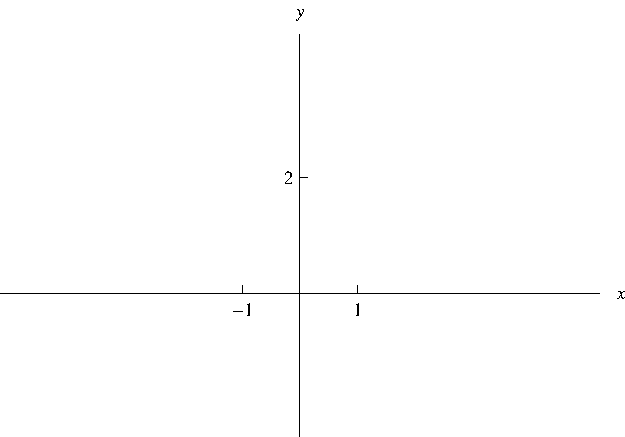
\includegraphics[width=5cm]{curve-sketching/pictures/04-05-ex1a.pdf}%
\psset{xunit=0.25cm, yunit=0.25cm}
\begin{pspicture}(-5, -5)(5,5) 
\psframe*[linecolor=white](-10,-10)(11,10) 
\tiny 
\psaxes[ticks=none, labels=none]{<->}(0,0)(-10,-4.5)(10,7)
\psline[linecolor=red!1](1,9)(1,9.001)
\psline[linecolor=red!1](1,-5.2)(1,-5.201)

\psLabels{10}{7}
\psXTickWithLabel{1}{$1$}
\psXTickWithLabel{-1}{$-1$}
\psYTickWithLabel{2}{$2$}
\psline[linecolor=red!1](1,9)(1,9.001)
%Function formula: \frac{2 x^{2}}{x^{2}-1} 
%\psplot[linecolor=\psColorGraph, plotpoints=1000]{1.15}{9.9}{x 2 exp 2 mul -1 x 2 exp add div }
%\psplot[linecolor=\psColorGraph, plotpoints=1000]{-0.85}{0.85}{x 2 exp 2 mul -1 x 2 exp add div }
%\psplot[linecolor=\psColorGraph, plotpoints=1000]{-9.9}{-1.15}{x 2 exp 2 mul -1 x 2 exp add div }
\end{pspicture}
 
\invisible<1->{
\abovedisplayskip=0pt
\belowdisplayskip=0pt
\[
\begin{array}{|@{}c@{}|c@{}|c@{}|}
\hline
\textrm{Interval}&\textrm{I/D}&\textrm{Concavity}\\
\hline
(-\infty , -1)&%
\textrm{I}&\\%
(-1 , 0)&%
\textrm{D}&\\%
(0 , 1)&%
\textrm{D}&\\%
(1 , \infty)&%
\textrm{I}&\\%
\hline
\end{array}
\]
}
\column{.55\textwidth}
\begin{enumerate}
\item<2->  Domain
\end{enumerate}
\uncover<2->{%
The domain of the function is \uncover<3->{\alert<handout:0| 3>{$(-\infty , -1) \cup (-1, 1)\cup (1,\infty )$}.}
}%
\end{columns}
\end{example}
\end{frame}






\begin{frame}[t]
\begin{example} %[Example 1, p. 245]
\begin{columns}[t]
\column{.45\textwidth}
Sketch the curve $y = \frac{2x^2}{x^2-1}$.
\psset{xunit=0.25cm, yunit=0.25cm}
\begin{pspicture}(-5, -5)(5,5) 
\psframe*[linecolor=white](-10,-10)(11,10) 
\tiny 
\psaxes[ticks=none, labels=none]{<->}(0,0)(-10,-4.5)(10,7)
\psline[linecolor=red!1](1,9)(1,9.001)
\psline[linecolor=red!1](1,-5.2)(1,-5.201)

\psLabels{10}{7}
\psXTickWithLabel{1}{$1$}
\psXTickWithLabel{-1}{$-1$}
\psYTickWithLabel{2}{$2$}
\uncover<7->{
\psFullDot{0}{0}
}
\end{pspicture}
%\ \only<handout:0| -5>{%
%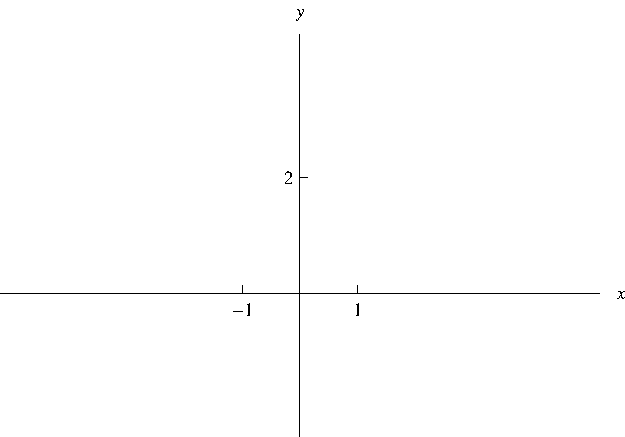
\includegraphics[width=5cm]{curve-sketching/pictures/04-05-ex1a.pdf}%
%}%
%\only<6->{%
%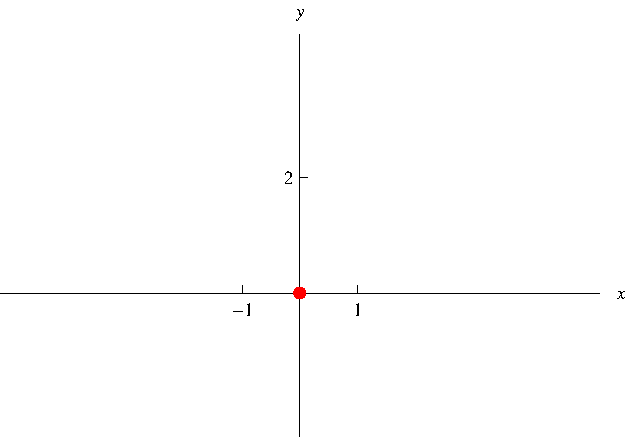
\includegraphics[width=5cm]{curve-sketching/pictures/04-05-ex1b.pdf}%
%}%

\invisible<1->{
\abovedisplayskip=0pt
\belowdisplayskip=0pt
\[
\begin{array}{|@{}c@{}|c@{}|c@{}|}
\hline
\textrm{Interval}&\textrm{I/D}&\textrm{Concavity}\\
\hline
(-\infty , -1)&%
\textrm{I}&\\%
(-1 , 0)&%
\textrm{D}&\\%
(0 , 1)&%
\textrm{D}&\\%
(1 , \infty)&%
\textrm{I}&\\%
\hline
\end{array}
\]
}
\column{.55\textwidth}
\begin{enumerate}
\setcounter{enumi}{2}
\item  Intercepts
\end{enumerate}
\begin{itemize}
\item<2-| alert@2-3>  $y$-intercept: $f(0) = $ \uncover<3->{$0$.}
\item<2-| alert@4-5>  $x$-intercept: $f(x) = 0$ when $x = $ \uncover<5->{$0$.}
\item<6->  The only intercept is $\alert<7>{(0,0)}$.
\end{itemize}
\end{columns}
\end{example}
\end{frame}


\begin{frame}[t]
\begin{example} %[Example 1, p. 245]
\begin{columns}[t]
\column{.45\textwidth}
Sketch the curve $y = \frac{2x^2}{x^2-1}$.
\psset{xunit=0.25cm, yunit=0.25cm}
\begin{pspicture}(-5, -5)(5,5) 
\psframe*[linecolor=white](-10,-10)(11,10) 
\tiny 
\psaxes[ticks=none, labels=none]{<->}(0,0)(-10,-4.5)(10,7)
\psline[linecolor=red!1](1,9)(1,9.001)
\psline[linecolor=red!1](1,-5.2)(1,-5.201)

\psLabels{10}{7}
\psXTickWithLabel{1}{$1$}
\psXTickWithLabel{-1}{$-1$}
\psYTickWithLabel{2}{$2$}
\psFullDot{0}{0}
\end{pspicture}

%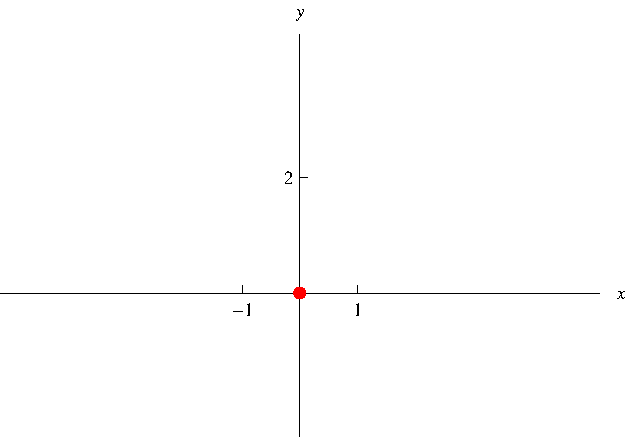
\includegraphics[width=5cm]{curve-sketching/pictures/04-05-ex1b.pdf}%

\invisible<1->{
\abovedisplayskip=0pt
\belowdisplayskip=0pt
\[
\begin{array}{|@{}c@{}|c@{}|c@{}|}
\hline
\textrm{Interval}&\textrm{I/D}&\textrm{Concavity}\\
\hline
(-\infty , -1)&%
\textrm{I}&\\%
(-1 , 0)&%
\textrm{D}&\\%
(0 , 1)&%
\textrm{D}&\\%
(1 , \infty)&%
\textrm{I}&\\%
\hline
\end{array}
\]
}
\column{.55\textwidth}
\begin{enumerate}
\setcounter{enumi}{3}
\item  Symmetry
\end{enumerate}
\[
\uncover<2->{%
f(-x) = \alert<handout:0| 3-4>{\frac{2(-x)^2}{(-x)^2-1}} %
}%
\uncover<3->{%
\alert<handout:0| 3-4>{ = \uncover<4->{\frac{2x^2}{x^2-1}}} %
}%
\uncover<5->{%
 = f(x)
}%
\]
\uncover<6->{Therefore $f$ is \uncover<7->{\alert<handout:0| 7>{even}.}}
\end{columns}
\end{example}
\end{frame}


\begin{frame}[t]
\begin{example} %[Example 1, p. 245]
\begin{columns}[t]
\column{.45\textwidth}
Sketch the curve $y = \frac{2x^2}{x^2-1}$.
\psset{xunit=0.25cm, yunit=0.25cm}
\begin{pspicture}(-5, -5)(5,5) 
\psframe*[linecolor=white](-10,-10)(11,10) 
\tiny 
\psaxes[ticks=none, labels=none]{<->}(0,0)(-10,-4.5)(10,7)
\psline[linecolor=red!1](1,9)(1,9.001)
\psline[linecolor=red!1](1,-5.2)(1,-5.201)

\psLabels{10}{7}
\uncover<1-14>{
\psXTickWithLabel{1}{$1$}
\psXTickWithLabel{-1}{$-1$}
}
\uncover<1-4>{
\psYTickWithLabel{2}{$2$}
}
\psFullDot{0}{0}
\uncover<5->{
\psline[linestyle=dashed, linewidth=0.3pt](-9.97,2 )(9.97,2)
\rput[t](-8.5, 1.9){$y=2$}
}
\uncover<4->{ %
\psplot[arrows=->,linecolor=\psColorGraph, plotpoints=1000]{8}{9.9}{x 2 exp 2 mul -1 x 2 exp add div }
} %
\uncover<8->{ %
\psplot[arrows=<-,linecolor=\psColorGraph, plotpoints=1000]{1.2}{1.8}{x 2 exp 2 mul -1 x 2 exp add div }
} %
\uncover<10->{
\psplot[arrows=->, linecolor=\psColorGraph, plotpoints=1000]{0.65}{0.8}{x 2 exp 2 mul -1 x 2 exp add div }
}
\uncover<12->{
\psplot[arrows=<-, linecolor=\psColorGraph, plotpoints=1000]{-0.8}{-0.65}{x 2 exp 2 mul -1 x 2 exp add div }
}

\uncover<4->{ %
\psplot[arrows=<-, linecolor=\psColorGraph, plotpoints=1000]{-9.9}{-8}{x 2 exp 2 mul -1 x 2 exp add div }
} %
\uncover<14->{ %
\psplot[arrows=->, linecolor=\psColorGraph, plotpoints=1000]{-1.8}{-1.2}{x 2 exp 2 mul -1 x 2 exp add div }
} %
\uncover<15->{ %
\psline[linestyle=dashed, linewidth=0.3pt](-1,-5)(-1,8)
\rput[r](-1.4, -3.5){$x=-1$}
\psline[linestyle=dashed, linewidth=0.3pt](1,-5)(1,8)
\rput[l](1.4, -3.5){$x=1$}
} %
\end{pspicture}

%\ \only<handout:0| -3>{%
%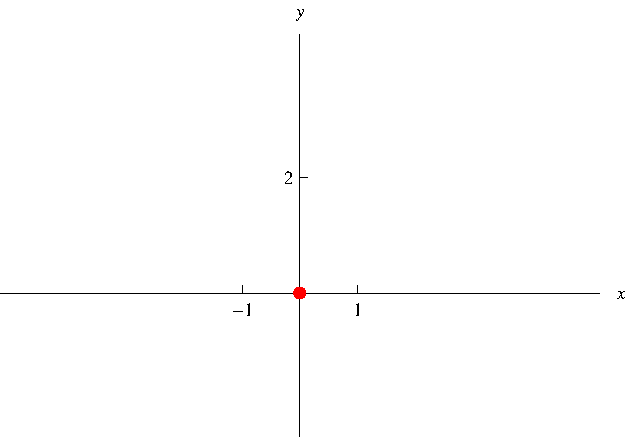
\includegraphics[width=5cm]{curve-sketching/pictures/04-05-ex1b.pdf}%
%}%
%\only<handout:0| 4>{%
%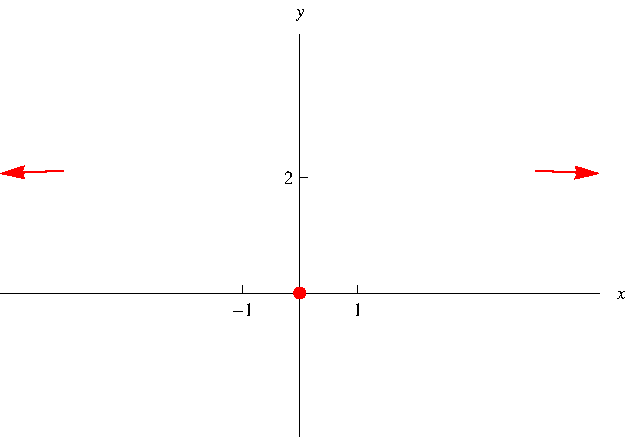
\includegraphics[width=5cm]{curve-sketching/pictures/04-05-ex1c.pdf}%
%}%
%\only<handout:0| 5-7>{%
%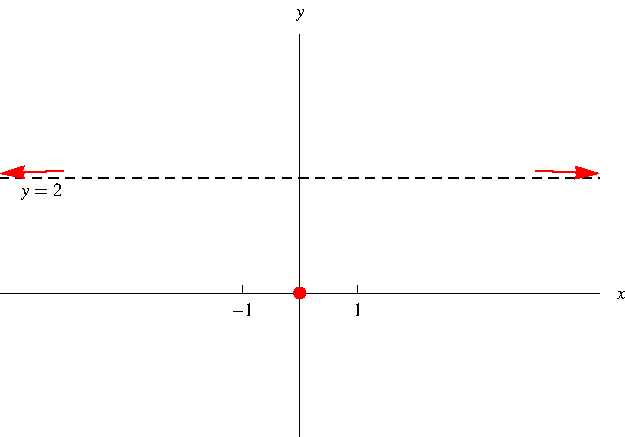
\includegraphics[width=5cm]{curve-sketching/pictures/04-05-ex1d.pdf}%
%}%
%\only<handout:0| 8-9>{%
%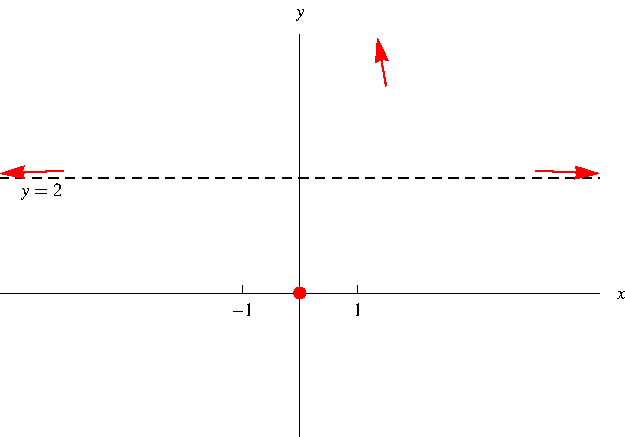
\includegraphics[width=5cm]{curve-sketching/pictures/04-05-ex1e.pdf}%
%}%
%\only<handout:0| 10-11>{%
%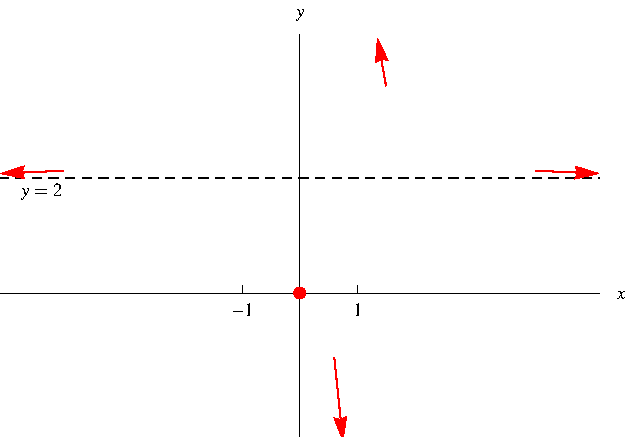
\includegraphics[width=5cm]{curve-sketching/pictures/04-05-ex1f.pdf}%
%}%
%\only<handout:0| 12-13>{%
%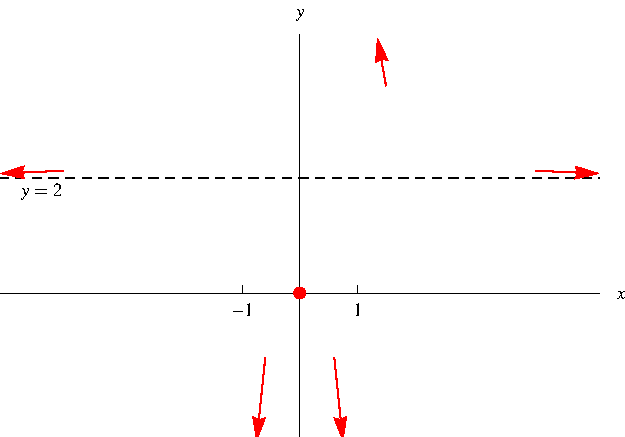
\includegraphics[width=5cm]{curve-sketching/pictures/04-05-ex1g.pdf}%
%}%
%\only<handout:0| 14>{%
%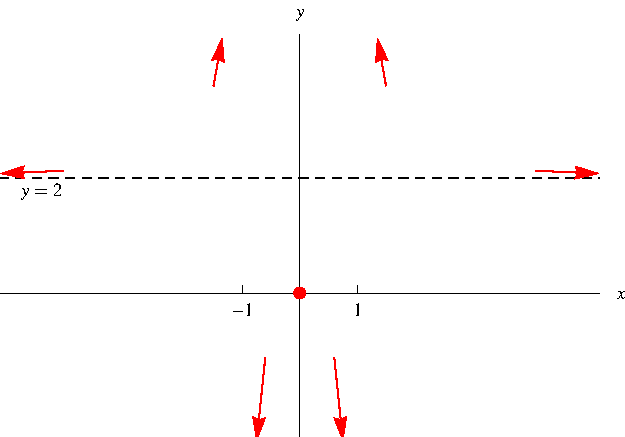
\includegraphics[width=5cm]{curve-sketching/pictures/04-05-ex1h.pdf}%
%}%
%\only<15->{%
%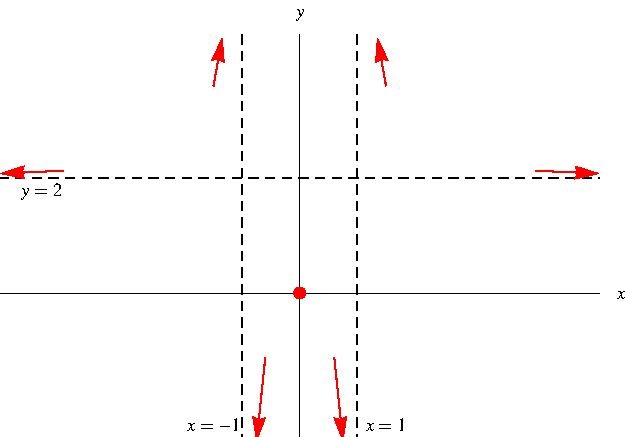
\includegraphics[width=5cm]{curve-sketching/pictures/04-05-ex1i.pdf}%
%}%

\invisible<1->{
\abovedisplayskip=0pt
\belowdisplayskip=0pt
\[
\begin{array}{|@{}c@{}|c@{}|c@{}|}
\hline
\textrm{Interval}&\textrm{I/D}&\textrm{Concavity}\\
\hline
(-\infty , -1)&%
\textrm{I}&\\%
(-1 , 0)&%
\textrm{D}&\\%
(0 , 1)&%
\textrm{D}&\\%
(1 , \infty)&%
\textrm{I}&\\%
\hline
\end{array}
\]
}

\column{.55\textwidth}
\begin{enumerate}
\setcounter{enumi}{4}
\item  Asymptotes
\end{enumerate}
\abovedisplayskip=0pt
\belowdisplayskip=0pt
\[
\uncover<2->{%
\lim_{x\to\pm\infty}\frac{2x^2}{x^2-1}%
}%
\uncover<3->{%
 = \lim_{x\to\pm\infty}\frac{2}{1 - 1/x^2}%
}%
\uncover<4->{%
 = 2%
}%
\]
\uncover<5->{$y = 2$ is a horizontal asymptote.}
\uncover<6->{%
\abovedisplayskip=0pt
\belowdisplayskip=0pt
\[
\begin{array}{r@{}c@{}l}
\displaystyle \alert<handout:0| 7-8>{\lim_{x\to 1^+}\frac{2x^2}{x^2-1}} & \alert<handout:0| 7-8>{=} & \uncover<8->{\alert<handout:0| 8>{\infty}} \\%
\displaystyle \alert<handout:0| 9-10>{\lim_{x\to 1^-}\frac{2x^2}{x^2-1}} & \alert<handout:0| 9-10>{=} & \uncover<10->{\alert<handout:0| 10>{-\infty}} \\%
\displaystyle \alert<handout:0| 11-12>{\lim_{x\to -1^+}\frac{2x^2}{x^2-1}} & \alert<handout:0| 11-12>{=} & \uncover<12->{\alert<handout:0| 12>{-\infty}} \\%
\displaystyle \alert<handout:0| 13-14>{\lim_{x\to -1^-}\frac{2x^2}{x^2-1}} & \alert<handout:0| 13-14>{=} & \uncover<14->{\alert<handout:0| 14>{\infty}} %
\end{array}
\]
}%
\uncover<15->{%
$x = \pm 1$ are vertical asymptotes.%
}%
\end{columns}
\end{example}
\end{frame}


\begin{frame}[t]
\begin{example} %[Example 1, p. 245]
\begin{columns}[t]
\column{.45\textwidth}
Sketch the curve $y = \frac{2x^2}{x^2-1}$.
\psset{xunit=0.25cm, yunit=0.25cm}
\begin{pspicture}(-5, -5)(5,5) 
\psframe*[linecolor=white](-10,-10)(11,10) 
\tiny 
\psaxes[ticks=none, labels=none]{<->}(0,0)(-10,-4.5)(10,7)
\psline[linecolor=red!1](1,9)(1,9.001)
\psline[linecolor=red!1](1,-5.2)(1,-5.201)

\psLabels{10}{7}
\psFullDot{0}{0}
\psline[linestyle=dashed, linewidth=0.3pt](-9.97,2 )(9.97,2)
\rput[t](-8.5, 1.9){$y=2$}
\psplot[arrows=->,linecolor=\psColorGraph, plotpoints=1000]{8}{9.9}{x 2 exp 2 mul -1 x 2 exp add div }
\psplot[arrows=<-,linecolor=\psColorGraph, plotpoints=1000]{1.2}{1.8}{x 2 exp 2 mul -1 x 2 exp add div }
\psplot[arrows=->, linecolor=\psColorGraph, plotpoints=1000]{0.65}{0.8}{x 2 exp 2 mul -1 x 2 exp add div }
\psplot[arrows=<-, linecolor=\psColorGraph, plotpoints=1000]{-0.8}{-0.65}{x 2 exp 2 mul -1 x 2 exp add div }
\psplot[arrows=<-, linecolor=\psColorGraph, plotpoints=1000]{-9.9}{-8}{x 2 exp 2 mul -1 x 2 exp add div }
\psplot[arrows=->, linecolor=\psColorGraph, plotpoints=1000]{-1.8}{-1.2}{x 2 exp 2 mul -1 x 2 exp add div }
\psline[linestyle=dashed, linewidth=0.3pt](-1,-5)(-1,8)
\rput[r](-1.4, -3.5){$x=-1$}
\psline[linestyle=dashed, linewidth=0.3pt](1,-5)(1,8)
\rput[l](1.4, -3.5){$x=1$}
\end{pspicture}

%\ \only<1->{%
%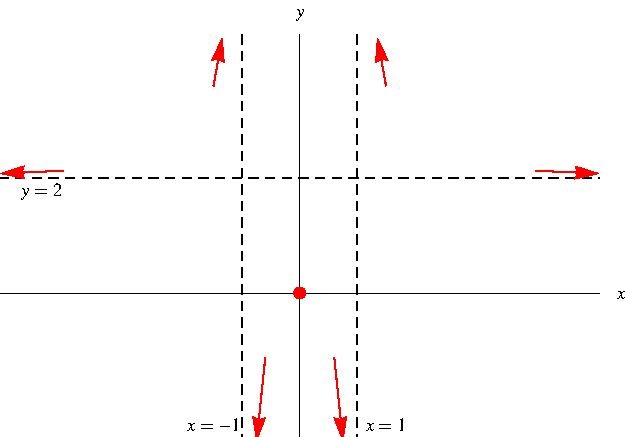
\includegraphics[width=5cm]{curve-sketching/pictures/04-05-ex1i.pdf}%
%}%

\abovedisplayskip=0pt
\belowdisplayskip=0pt
\[
\begin{array}{|@{}c@{}|c@{}|c@{}|}
\hline
\textrm{Interval}&\alert<handout:0| 12>{\textrm{I/D}}&\textrm{Concavity}\\
\hline
(-\infty , -1)&%
\uncover<12->{\alert<handout:0| 12>{\textrm{I}}}&\\%
(-1 , 0)&%
\uncover<12->{\alert<handout:0| 12>{\textrm{I}}}&\\%
(0 , 1)&%
\uncover<12->{\alert<handout:0| 12>{\textrm{D}}}&\\%
(1 , \infty)&%
\uncover<12->{\alert<handout:0| 12>{\textrm{D}}}&\\%
\hline
\end{array}
\]

\column{.55\textwidth}
\begin{enumerate}
\setcounter{enumi}{5}
\item  Intervals of increase or decrease
\end{enumerate}
\abovedisplayskip=0pt
\belowdisplayskip=0pt
\begin{eqnarray*}
\uncover<2->{%
\alert<handout:0| 3-4>{f'(x)}% 
}%
& \uncover<2->{\alert<handout:0| 3-4>{ = }} &%
\uncover<4->{%
\alert<handout:0| 4>{\frac{(x^2-1)(4x) - 2x^2(2x)}{(x^2-1)^2}}%
}\\%
&\uncover<5->{ = } &%
\uncover<5->{%
 \frac{-4x}{(x^2-1)^2}%
}%
\end{eqnarray*}
\uncover<6->{%
\[
\begin{array}{|c@{}|c@{}|c@{}|c@{}|}
\hline
& \alert<handout:0| 7-8>{-4x} & \alert<handout:0| 9-10>{(x^2-1)^2} & \alert<handout:0| 11>{f'} \\
\hline
(-\infty , -1) & \alert<handout:0| 7-8>{\uncover<8->{+}} & \alert<handout:0| 9-10>{\uncover<10->{+}} & \alert<handout:0| 11>{\uncover<11->{+}} \\
(-1 , 0) & \alert<handout:0| 7-8>{\uncover<8->{+}} & \alert<handout:0| 9-10>{\uncover<10->{+}} & \alert<handout:0| 11>{\uncover<11->{+}} \\
(0 , 1) & \alert<handout:0| 7-8>{\uncover<8->{-}} & \alert<handout:0| 9-10>{\uncover<10->{+}} & \alert<handout:0| 11>{\uncover<11->{-}} \\
(1 , \infty) & \alert<handout:0| 7-8>{\uncover<8->{-}} & \alert<handout:0| 9-10>{\uncover<10->{+}} & \alert<handout:0| 11>{\uncover<11->{-}} \\
\hline
\end{array}
\]
}%
\end{columns}
\end{example}
\end{frame}


\begin{frame}[t]
\begin{example} %[Example 1, p. 245]
\begin{columns}[t]
\column{.45\textwidth}
Sketch the curve $y = \frac{2x^2}{x^2-1}$.
\psset{xunit=0.25cm, yunit=0.25cm}
\begin{pspicture}(-5, -5)(5,5) 
\psframe*[linecolor=white](-10,-10)(11,10) 
\tiny 
\psaxes[ticks=none, labels=none]{<->}(0,0)(-10,-4.5)(10,7)
\psline[linecolor=red!1](1,9)(1,9.001)
\psline[linecolor=red!1](1,-5.2)(1,-5.201)

\psLabels{10}{7}
\psFullDot{0}{0}
\psline[linestyle=dashed, linewidth=0.3pt](-9.97,2 )(9.97,2)
\rput[t](-8.5, 1.9){$y=2$}
\psplot[arrows=->,linecolor=\psColorGraph, plotpoints=1000]{8}{9.9}{x 2 exp 2 mul -1 x 2 exp add div }
\psplot[arrows=<-,linecolor=\psColorGraph, plotpoints=1000]{1.2}{1.8}{x 2 exp 2 mul -1 x 2 exp add div }
\psplot[arrows=->, linecolor=\psColorGraph, plotpoints=1000]{0.65}{0.8}{x 2 exp 2 mul -1 x 2 exp add div }
\psplot[arrows=<-, linecolor=\psColorGraph, plotpoints=1000]{-0.8}{-0.65}{x 2 exp 2 mul -1 x 2 exp add div }
\psplot[arrows=<-, linecolor=\psColorGraph, plotpoints=1000]{-9.9}{-8}{x 2 exp 2 mul -1 x 2 exp add div }
\psplot[arrows=->, linecolor=\psColorGraph, plotpoints=1000]{-1.8}{-1.2}{x 2 exp 2 mul -1 x 2 exp add div }
\psline[linestyle=dashed, linewidth=0.3pt](-1,-5)(-1,8)
\rput[r](-1.4, -3.5){$x=-1$}
\psline[linestyle=dashed, linewidth=0.3pt](1,-5)(1,8)
\rput[l](1.4, -3.5){$x=1$}
\end{pspicture}

%\ \only<1->{%
%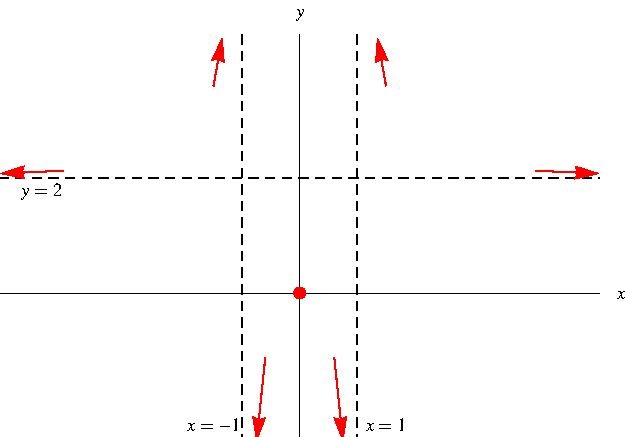
\includegraphics[width=5cm]{curve-sketching/pictures/04-05-ex1i.pdf}%
%}%

\abovedisplayskip=0pt
\belowdisplayskip=0pt
\[
\begin{array}{|@{}c@{}|c@{}|c@{}|}
\hline
\textrm{Interval}&\textrm{I/D}&\textrm{Concavity}\\
\hline
(-\infty , -1)&%
\textrm{I}&\\%
(-1 , 0)&%
\textrm{I}&\\%
(0 , 1)&%
\textrm{D}&\\%
(1 , \infty)&%
\textrm{D}&\\%
\hline
\end{array}
\]

\column{.55\textwidth}
\begin{enumerate}
\setcounter{enumi}{6}
\item  Local maxima and minima
\end{enumerate}
\[
\begin{array}{|c@{}|c@{}|c@{}|c@{}|}
\hline
& -4x & (x^2-1)^2 & f' \\
\hline
(-\infty , -1) & + & + & + \\
\alert<handout:0| 2>{(-1 , 0)} & + & + & \alert<handout:0| 2>{+} \\
\alert<handout:0| 2>{(0 , 1)} & - & + & \alert<handout:0| 2>{-} \\
(1 , \infty) & - & + & - \\
\hline
\end{array}
\]
\begin{itemize}
\item<2->  $f'$ changes sign from $+$ to $-$ at $0$.
\item<3->  Therefore $(0,0)$ is a local maximum.
\end{itemize}
\end{columns}
\end{example}
\end{frame}

\begin{frame}[t]
\begin{example} %[Example 1, p. 245]
\begin{columns}[t]
\column{.45\textwidth}
Sketch the curve $y = \frac{2x^2}{x^2-1}$.
\psset{xunit=0.25cm, yunit=0.25cm}
\begin{pspicture}(-5, -5)(5,5) 
\psframe*[linecolor=white](-10,-10)(11,10) 
\tiny 
\psaxes[ticks=none, labels=none]{<->}(0,0)(-10,-4.5)(10,7)
\psline[linecolor=red!1](1,9)(1,9.001)
\psline[linecolor=red!1](1,-5.2)(1,-5.201)

\psLabels{10}{7}
\psFullDot{0}{0}
\psline[linestyle=dashed, linewidth=0.3pt](-9.97,2 )(9.97,2)
\rput[t](-8.5, 1.9){$y=2$}
\psline[linestyle=dashed, linewidth=0.3pt](-1,-5)(-1,8)
\rput[r](-1.4, -3.5){$x=-1$}
\psline[linestyle=dashed, linewidth=0.3pt](1,-5)(1,8)
\rput[l](1.4, -3.5){$x=1$}
\uncover<1-13>{ %
\psplot[arrows=->,linecolor=\psColorGraph, plotpoints=1000]{8}{9.9}{x 2 exp 2 mul -1 x 2 exp add div }
\psplot[arrows=<-,linecolor=\psColorGraph, plotpoints=1000]{1.2}{1.8}{x 2 exp 2 mul -1 x 2 exp add div }
\psplot[arrows=->, linecolor=\psColorGraph, plotpoints=1000]{0.65}{0.8}{x 2 exp 2 mul -1 x 2 exp add div }
\psplot[arrows=<-, linecolor=\psColorGraph, plotpoints=1000]{-0.8}{-0.65}{x 2 exp 2 mul -1 x 2 exp add div }
\psplot[arrows=<-, linecolor=\psColorGraph, plotpoints=1000]{-9.9}{-8}{x 2 exp 2 mul -1 x 2 exp add div }
\psplot[arrows=->, linecolor=\psColorGraph, plotpoints=1000]{-1.8}{-1.2}{x 2 exp 2 mul -1 x 2 exp add div }
}
\uncover<14->{ %
\psplot[linecolor=\psColorGraph, plotpoints=1000]{1.15}{9.9}{x 2 exp 2 mul -1 x 2 exp add div }
\psplot[linecolor=\psColorGraph, plotpoints=1000]{-0.85}{0.85}{x 2 exp 2 mul -1 x 2 exp add div }
\psplot[linecolor=\psColorGraph, plotpoints=1000]{-9.9}{-1.15}{x 2 exp 2 mul -1 x 2 exp add div }
} %
\end{pspicture}
%\ \only<handout:0| -13>{%
%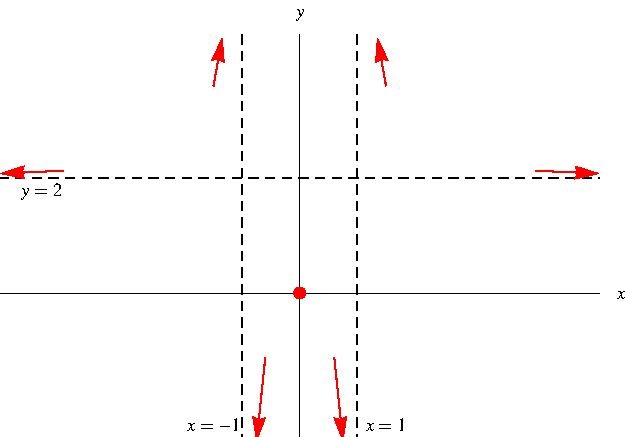
\includegraphics[width=5cm]{curve-sketching/pictures/04-05-ex1i.pdf}%
%}%
%\only<14->{%
%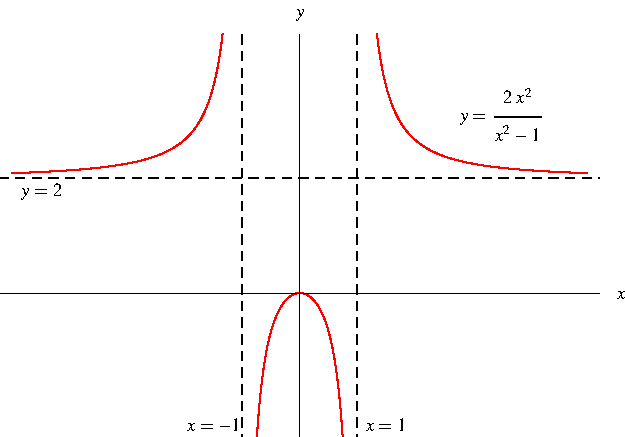
\includegraphics[width=5cm]{curve-sketching/pictures/04-05-ex1j.pdf}%
%}%

\abovedisplayskip=0pt
\belowdisplayskip=0pt
\[
\begin{array}{|@{}c@{}|c@{}|c@{}|}
\hline
\textrm{Interval}&\textrm{I/D}&\alert<handout:0| 12>{\textrm{Concavity}}\\
\hline
(-\infty , -1)&%
\textrm{I}&\uncover<12->{\alert<handout:0| 12>{\textrm{up}}}\\%
(-1 , 0)&%
\textrm{I}&\uncover<12->{\alert<handout:0| 12>{\textrm{down}}}\\%
(0 , 1)&%
\textrm{D}&\uncover<12->{\alert<handout:0| 12>{\textrm{down}}}\\%
(1 , \infty)&%
\textrm{D}&\uncover<12->{\alert<handout:0| 12>{\textrm{up}}}\\%
\hline
\end{array}
\]

\column{.55\textwidth}
\begin{enumerate}
\setcounter{enumi}{7}
\item  Concavity and points of inflection
\end{enumerate}
\abovedisplayskip=0pt
\belowdisplayskip=0pt
\begin{eqnarray*}
& & \uncover<2->{%
\ \ \alert<handout:0| 3-4>{f''(x)}% 
}\\%
%& \uncover<2->{\alert<handout:0| 3-4>{ = }} &%
&&\uncover<4->{%
\alert<handout:0| 4>{ = \frac{-4(x^2-1)^2+4x\cdot 2(x^2-1)2x}{(x^2-1)^4}}%
}\\%
%&\uncover<5->{ = } &%
&&\uncover<5->{%
 =  \frac{12x^2+4}{(x^2-1)^3}%
}%
\end{eqnarray*}
\uncover<6->{%
\[
\begin{array}{|@{}c@{}|c@{}|c@{}|c@{}|}
\hline
& \alert<handout:0| 7-8>{12x^2+4} & \alert<handout:0| 9-10>{(x^2-1)^3} & \alert<handout:0| 11>{f''} \\
\hline
(-\infty , -1) & \alert<handout:0| 7-8>{\uncover<8->{+}} & \alert<handout:0| 9-10>{\uncover<10->{+}} & \alert<handout:0| 11>{\uncover<11->{+}} \\
(-1 , 1) & \alert<handout:0| 7-8>{\uncover<8->{+}} & \alert<handout:0| 9-10>{\uncover<10->{-}} & \alert<handout:0| 11>{\uncover<11->{-}} \\
(1 , \infty) & \alert<handout:0| 7-8>{\uncover<8->{+}} & \alert<handout:0| 9-10>{\uncover<10->{+}} & \alert<handout:0| 11>{\uncover<11->{+}} \\
\hline
\end{array}
\]
}%
\uncover<13,14->{%
No points of inflection because $\pm 1$ are not in the domain of $f$.
}%
\end{columns}
\end{example}
\end{frame}
% end module curve-sketching-guidelines-ex1
